\chapter{State of art}
\label{chp:state}

In this section, we present previous works that also aim at
supporting the development of multimodal (\sect{sec:state:multimodal}) and
multiuser (\sect{sec:state:multiuser}) interactions. Then, we summarize their
drawbacks (\sect{sec:state:drawbacks}).

\section{Support for multimodal interactions}
\label{sec:state:multimodal}

In order to guide our discussion about the support of multimodal interactions,
we present Dumas’s abstract architecture for MUI systems
~\cite{dumas_multimodal_2009} in what follows.

Dumas’s architecture (illustrated in \fig{fig:dulmas}) presents a MUI as a
perceptions-actions cycle between the multimodal system and the user. The user
performs actions through human communication activities (\textit{e.g.} speech, gestures,
touch) and perceives the (result of) system actions through stimuli to her/his
senses (\textit{e.g.} sight, hearing). We detail the key components of the architecture in
what follows.

\begin{figure}[!ht]
\begin{center}
	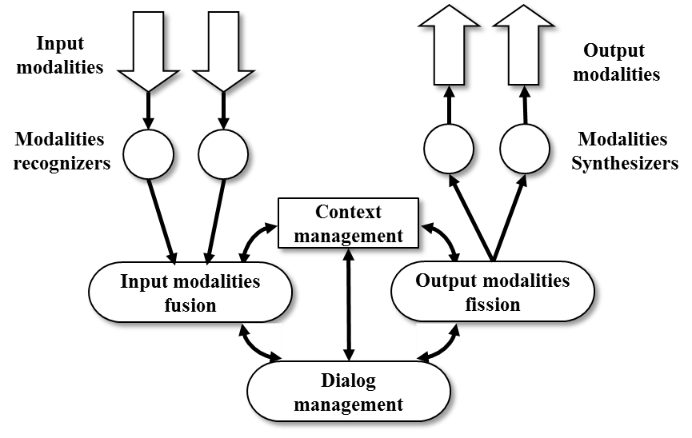
\includegraphics[width=10cm, keepaspectratio]{img/img6.png}
	\caption[Conceptual architecture of a multimodal system]{Conceptual
	architecture of a multimodal system, adapted from~\cite{dumas_multimodal_2009}.}
	\label{fig:dulmas}
    \captionvspace
\end{center}
\end{figure}

\textit{Modalities recognizers} are capable of decoding \textit{input
modalities} through input devices and sensors (\textit{e.g.} keyboard, video camera, and
microphone). For example, an ASR (Audio Speech Recognition) recognizer
identifies sentences in audio samples captured by a microphone.
\textit{Modalities synthesizers} are capable of producing \textit{output
modalities} through audiovisual output devices and actuator devices (\textit{e.g.}~
monitor, speakers, haptic). For instance, a TTS (Text-To-Speech) synthesizer
produces audio to be played by a speaker.

\textit{Input modalities fusion} is the process of combining the recognizers’
results to interpret the user actions. For instance, fusion should interpret a
user text conveyed in either a speech or an ink modality. In addition, the
fusion should consider contextual information; for instance, it should not
expect voice commands from a speech-impaired user or when the user is in a loud
environment.

\textit{Output modalities fission} is the generation of a system message --a
combination of actions in one or more synthesizers-- conveyed to the user
through certain output modalities. The choice of which modalities are used in
the message is called \textit{modality selection}, which must also consider
contextual information —\textit{e.g.} it would not make sense to use visual modalities to
convey information to a blind user.

\textit{Dialog management} maintains the communication flow between the user
and the system. The dialog defines a combination of fission and fusion
processes, performed at each moment of application behavior. Finally,
\textit{context management} is responsible for storing the user context
(\textit{e.g.} car, mobile, home) and profile (\textit{e.g.} blind, deaf,
mute), which enables the fission and fusion processes to be adapted. In view
the of Dumas’s architecture, we discuss four groups of works in the next
subsections (from \ref{sec:state:monomodal} to \ref{sec:state:multimedia}). As
illustrated in \tab{table:state}, each group supports some parts of the Dumas’s
architecture.

\begin{landscape}
\centering
\begin{table}
\scriptsize
\def\arraystretch{2}
%\resizebox{24cm}{!}{%
\begin{tabular}[]{ m{4cm}|m{3cm} m{3cm} m{3cm} m{3cm} m{3cm} m{3cm}}

	%%%%%%
	\hline
	\textbf{Approach}
		& \textbf{Recognizers}
		& \textbf{Fusion}
		& \textbf{Dialog \newline management}
		& \textbf{Context \newline management}
		& \textbf{Fission}
		& \textbf{Synthesizers} \\
	\hline

	%%%%%%
	\hline
	\rowcolor[HTML]{F2F2F2} \multicolumn{7}{c}{Language used by either
	recognizers or synthesizers}\\
	\hline

	\textbf{SRGS~\cite{andrew_hunt_speech_2004}, InkXML~\cite{w3c_ink_2011}, GDL~\cite{hachaj_semantic_2012}, and GML~\cite{ideum_inc_gesture_2016}} &
	specialized
	modality & sequential-only & & & \\
	\textbf{SSML~\cite{daniel_c._burnett_speech_2010},
	BML~\cite{vilhjalmsson_behavior_2007}, and
	SEDL~\cite{iso/iec_iso/iec_2013}} & & & & & specialized
	modality &
	sequential-only\\
	\hline

	%%%%%%
	\rowcolor[HTML]{F2F2F2} \multicolumn{7}{c}{Form-based dialog languages}\\
	\hline

	\textbf{VoiceXML~\cite{w3c_voice_2007} and SALT
	~\cite{microsoft_speech_2003}} & speech & sequential-only &
	form-based & & sequential-only & speech \\
	\textbf{XISL~\cite{katsurada_xisl:_2005}} & agnostic <input> element	&
	SMIL
	\textit{seq},\textit{par} and \textit{alt} operators & form-based & & SMIL
	seq, par and alt operators & agnostic <output> element \\
	\hline

	%%%%%%
	\hline
	\rowcolor[HTML]{F2F2F2} \multicolumn{7}{c}{Frameworks}\\
	\hline

	\textbf{MMI~\cite{w3c_multimodal_2003}} & MCs with LifeCycle messages & DoneNotification with EMMA
	& state machine\newline(SCXML) & SCXML \newline (ECMAScript) & sequence of
	LifeCycle messages (optionally inside if-then-else) & MCs with LifeCycle
	messages \\
	\textbf{HephaticsTK~\cite{dumas_description_2010}} & SMUIML \newline agnostic <recognizer> element &
	CARE properties based operators & state machine (SMUIML) & & SMUIML
	sequence of <result> elements & ad-hoc message\\
	\hline

	%%%%%%
	\hline
	\rowcolor[HTML]{F2F2F2} \multicolumn{7}{c}{Multimedia languages}\\
	\hline

	\textbf{HTML+SALT~\cite{wang_salt:_2002} and HTML+ VoiceXML~\cite{w3c_xhtml+voice_2001}} & key/pointer+
	VoiceXML & &
	low-level (JavaScript) & & & text, image, video, and audio elements\\
	\textbf{SMIL+Rex~\cite{beckham_towards_2001}} & key/pointer+ VoiceXML & & low-level (par and seq
	time
	containers) & & seq, par, excl time containers & text, image, video and
	audio elements\\
	\textbf{NCL+VoiceXML~\cite{carvalho_estendendo_2010}} & key/pointer+ VoiceXML & & low-level (causality
	links) & user and system variables & seq operators with media, switch, and
	anchors & agnostic media element\\
	\hline

\end{tabular}
%}
\caption{Comparison among the features supported by the different MUI
development approaches.}
\label{table:state}
\end{table}
\end{landscape}

\subsection{Languages used by recognizers and synthesizers}
\label{sec:state:monomodal}

The first group of related work consists of languages that handle either only
\textit{recognizers} or only \textit{synthesizers}. None of them supports dialog
or context management.

SRGS (Speech Recognition Grammar Specification)~\cite{andrew_hunt_speech_2004},
InkXML (Ink Markup Language)~\cite{w3c_ink_2011}, GDL (Gesture Description
Language)~\cite{hachaj_semantic_2012}, and GML (Gesture Markup Language)
~\cite{ideum_inc_gesture_2016} assist in describing \textit{recognizers}. SRGS
is a grammar format for speech recognition. InkXML is a representation for
electronic ink created with a stylus or other pointing devices, useful for
handling text input. Finally, GDL and GML focus on describing user movements:
GDL describes body joint movements captured by sensors (\textit{e.g.} Microsoft Kinect),
and GML focuses on touch gestures captured by touchpad devices.

SSML (Speech Synthesis Markup Language)~\cite{daniel_c._burnett_speech_2010},
BML (Behavior Markup Language)~\cite{vilhjalmsson_behavior_2007}, and SEDL
(Sensory Effect Description Language)~\cite{iso/iec_iso/iec_2013} assist in
describing \textit{synthesizers}. SSML is a representation for pronunciations
focused on text-to-speech engines and can control speech aspects (\textit{e.g.}~
pronunciation, volume, rate, pitch, and rhythm). BML enables controlling the
verbal and nonverbal behavior of embodied conversational, useful for children-
or elderly-oriented MUIs. Finally, SEDL, part of the MPEG-V framework
~\cite{iso/iec_iso/iec_2014}, supports the description of sensory effects such
as light, wind, fog, and chair vibration, which can be useful to enhance the
consumer’s experience of an audiovisual content.

\subsection{Form-based dialog languages}
\label{sec:state:dialog}

The second group of related work consists of languages that focus on specifying
the dialog management through a form-based approach. More precisely, developers
specify MUI systems through questions, to be conveyed by the system through
synthesizers, and expected answers from the user, interpreted through
recognizers. None of the works in this group supports context management.

VoiceXML (Voice Extensible Markup Language)~\cite{w3c_voice_2007} and SALT
(Speech Application Language Tags)~\cite{microsoft_speech_2003} are limited
to speech modalities and the widely used development of vocal interactions
focusing on telephony conversations. They can use synthesized speech and
digitized audio (voice recordings) as output. In addition, they can recognize
speech and telephony DTMF (Dual-Tone Multi-Frequency) digits as input. Both
focus on speech-only conversations, providing elements such as <listen> and
<prompt>. In those languages, the author only combines a sequence of input or a
sequence of output modalities.

XISL (eXtensible Interaction Scenario Language)~\cite{katsurada_xisl:_2005}
introduces an agnostic
treatment for modalities through the <input> and <output> elements. It is
inspired by the VoiceXML dialog but uses SMIL <par> and <seq> elements for
defining the modalities synchronization. The XISL dialog uses a <prompt> element
for system questions, <operation> for the fusion of user inputs, and <action>
for the fission of outputs —\textit{i.e.}~, the system response. Inside fusion (\textit{i.e.}~
<operation>) or fission (\textit{i.e.}~ <action>), XSI supports temporal relationships
through the <par> and <seq> SMIL elements, which are children of the <operation>
and <action> elements.

\subsection{Frameworks}
\label{sec:state:frameworks}

The third group of related work consists of frameworks that focus on specifying
the dialog management, usually using state machines. Those frameworks delegate
the fission to be handled by a multimedia system. For instance, fine media
synchronization, such as lip-syncs, are delegated to the multimedia system.

W3C’s MMI (Multimodal Interaction)~\cite{w3c_multimodal_2003} framework is
defined by Modality Components (MCs) and an Interaction Manager (IM). Inspired
by XISL, an MC is modality agnostic and it is responsible for one or more input
or output modalities, which it can handle by nesting other MCs and IMs. The IM
controls the dialog flow of the application by coordinating the MCs by message
exchange using an API named Life-Cycle~\cite{w3c_multimodal_2012}. These
messages include the activation of an MC (\textit{e.g.} Start, Pause, Cancel) and the
result of an MC by a DoneNotification (\textit{e.g.} end of speech recognition). MMI is
instantiated by \textit{control} and
\textit{presentation} documents, which implement IM and MCs, respectively. MMI
recommends the use of SCXML~\cite{w3c_state_2012} for control documents, and
VoiceXML, HTML, or SMIL for presentation documents. \fig{fig:mmi} illustrates
the message exchange between control and presentation documents. An SCXML
document describes the multimodal dialog using state machines, in which a set of
<state> and <transition> elements defines the possible states of the multimodal
application and the transitions between them. When transitioning between states,
SCXML sends life-cycle events to MCs. Additionally, these transitions can use
“if-then-else” constructions and ECMAScript variables. MMI recommends EMMA
(Extensible MultiModal Annotation markup language)~\cite{w3c_emma:_2009} to
describe DoneNotification messages exchanged between presentation documents and
their IM. EMMA defines a semantic interpretation for a variety of modalities;
for instance, presentation documents can interpret a text input in either a
speech or an ink modality.

\begin{figure}[!ht]
\begin{center}
	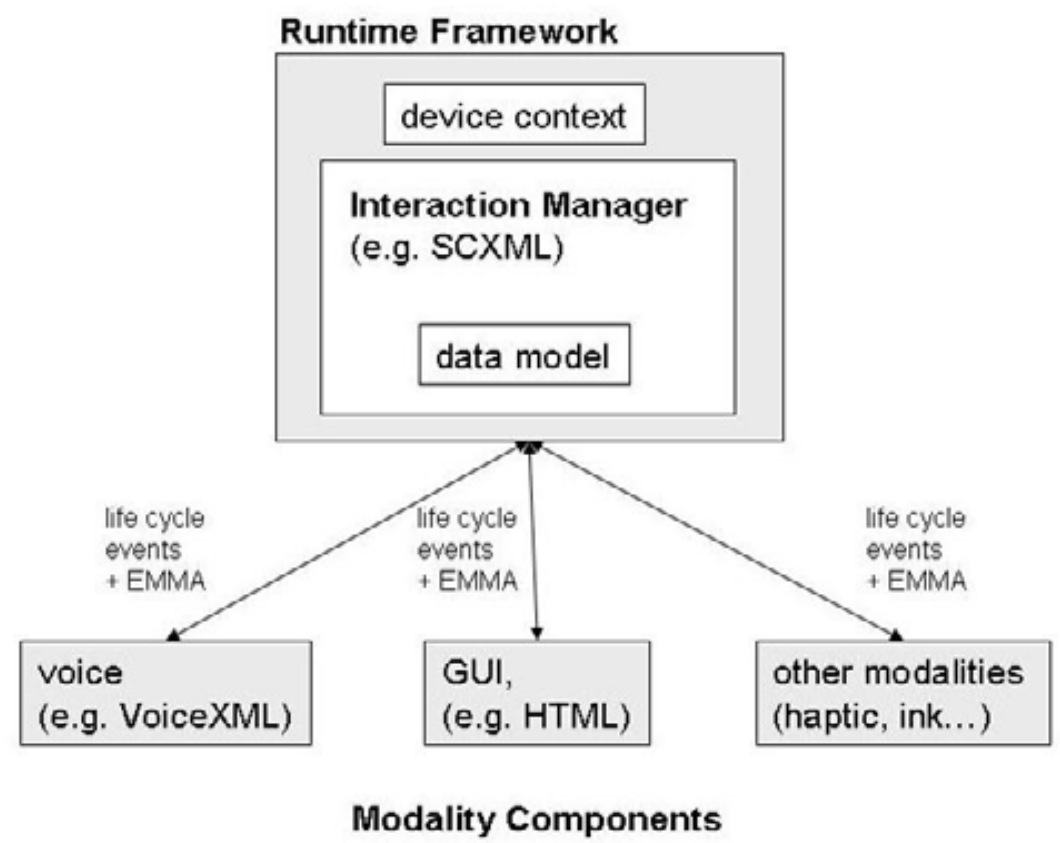
\includegraphics[width=5cm, keepaspectratio]{img/img7.png}
	\caption[MMI overview]{MMI overview, from~\cite{dahl_standards_2009}.}
	\label{fig:mmi}
	\captionvspace
\end{center}
\end{figure}

Aiming at implementing his architecture, Dumas proposes the HephaticsTK
framework. This framework is instantiated by one SMUIML (Synchronized
Multimodal User Interaction Modeling Language)~\cite{dumas_description_2010} document and its client
application. Illustrated in \fig{fig:smuiml}, SMUIML is a state-machine-based
language
that focuses on the specification of the fusion process. HephaticsTK delegates
the fission to the client application in charge of interpreting the message and
generating one or more output modalities.

\begin{figure}[!ht]
\begin{center}
	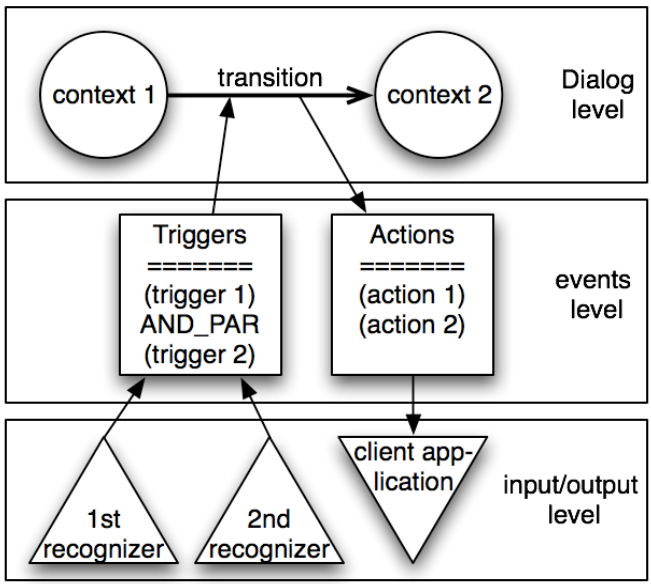
\includegraphics[width=5cm, keepaspectratio]{img/img8.png}
	\caption[SMUIML overview]{SMUIML overview, from~\cite{dumas_prototyping_2008}.}
	\label{fig:smuiml}
    \captionvspace
\end{center}
\end{figure}

In an SMUIML document, a state transition (<transition> element) is defined
through a combination of recognizers’ results (<triggers>) and messages to be
sent to the client application (<action>). This combination process of SMUIML
considers the CARE (\textit{Complementarity}, \textit{Assignment},
\textit{Redundancy}, and \textit{Equivalence}) properties~\cite{coutaz_four_1995}.

The formal expressions of the CARE properties rely on the transitions between
two states of a given multimodal system. Considering S’ following S,
\textit{Assignment} expresses the absence of choice: a single modality is
available in S to reach S’. \textit{Equivalence} means the availability of
choice between multiple modalities, \textit{i.e.}~, the use of any one of the modalities is
enough to reach state S’ from state S. \textit{Redundancy} means that a set of
modalities are used redundantly to reach S’ from S, \textit{i.e.}~, when they are used
within the same temporal window without increasing the user’s expressive power.
A set of modalities is used in a \textit{Complementary} way within a temporal
window if all of them must be used to reach S’ from S, either sequentially or in
parallel. \sect{sec:state:allen} discusses the state of the art in
terms of combination of modalities and their expressiveness.

SMUIML implements CARE assignment by using only one <trigger> per <transition>.
To implement the remainder CARE properties, SMUIML proposes four elements to
combine the <trigger>s: <par\_and> (CARE \textit{parallel Complementarity});
<seq\_and> (CARE \textit{sequential Complementarity}); <par\_or> (CARE
\textit{Redundancy}); and <seq\_or> (CARE \textit{Equivalence}).
\lis{list:smuiml} shows the “Put-that-there” in SMUIML, which uses <seq\_and>
and <par\_and> combinations.

\begin{listing}
\begin{minted}[linenos,fontsize=\scriptsize,numbersep=1pt,frame=lines,xleftmargin=10pt,framesep=2mm]{xml}
<transition leadtime="1500">
<seq_and>
  <trigger name="put_trigger" />
  <transition>
  <par_and>
    <trigger name="that_trigger" />
    <trigger name="object_pointed_event" />
  </par_and>
  </transition>
  <transition>
  <par_and>
    <trigger name="there_trigger" />
    <trigger name="object_pointed_event" />
  </par_and>
  </transition>
</seq_and>
<result action="put_that_there_action" />
</transition>
\end{minted}
\caption[“Put-that-there” expressed in SMUIML.]{“Put-that-there” example
illustrating CARE properties, expressed in
SMUIML. Adapted from~\cite{dumas_frameworks_2010}.}
\label{list:smuiml}
\end{listing}

\subsection{Multimedia languages}
\label{sec:state:multimedia}

Similar to our approach, some works
~\cite{beckham_towards_2001,carvalho_architectures_2008,
carvalho_estendendo_2010,	w3c_xhtml+voice_2001,wang_salt:_2002} extended XHTML
(eXtensible Hypertext Markup Language)~\cite{w3c_xhtml_2000}, SMIL, and NCL to
support multimodal interactions. The main drawback of these works, however, is
that they do not provide a way to seamlessly integrate new modalities, because
they incorporate recognizer specification by overloading existing elements or
adding directly into a multimedia language body. In particular, they are limited
to adding only a speech modality by incorporating VoiceXML and SALT elements.

Wang~\cite{wang_salt:_2002} proposes the integration of SALT elements
(\textit{e.g.} <salt:prompt>, <salt:grammar>) directly into XHTML. Likewise,
W3C~\cite{w3c_xhtml+voice_2001} proposes the integration of VoiceXML elements
(\textit{e.g.} <vxml:prompt>,<vxml:grammar>) directly into XHTML. Both proposals
use DOM events or JavaScript code to support relationships between voice
recognition/synthesis with XHTML content. Those scripts allow developers to
control, in an imperative manner, the activation of recognizers and
synthesizers, as well as the notification of the recognizers’ result.

Beckham~\cite{beckham_towards_2001} proposes elements for integrating voice
recognition and synthesis in SMIL. For speech synthesis, Beckman proposes a
<TTS:render> element. For speech recognition, Beckman proposes a reactive
language, named REX (Reactive XML), which has <raise>, <handle>, and <await> as
its main elements. The <raise> element specifies the ASR (Audio Speech
recognition) grammar to be recognized; <handle> defines actions that must be
performed when a recognition grammar is accepted; and <await> acts as a <par>
composition which includes <raise> and <handle>. As with other related work,
Beckman’s proposal merges elements related to recognition and speech synthesis
with the specification of the multimedia document. Another drawback is the fact
that it only adds supports to recognition and synthesis of a single modality
(voice).

Carvalho \textit{et al.}~\cite{carvalho_architectures_2008,carvalho_estendendo_2010}
propose two approaches for integrating VoiceXML elements into NCL. They both
incorporate VoiceXML directly into the XML tree of an NCL document and then map
VoiceXML elements for voice recognition onto keyboard-based events of NCL. In
~\cite{carvalho_architectures_2008}, a VoiceXML dialog is inserted into the
<port> NCL element (\lis{list:carvalho1}) and is activated in the beginning of
the document, whereas in~\cite{carvalho_estendendo_2010} the dialogue is
inserted into the <link> element (\lis{list:carvalho2}) and is activated when
the media related with the <link> is occurring. Besides overloading the concept
of the <port> and <link> elements, these approaches compromise the separation
between the structure and the content of the application, which is favored by
the NCL model, namely NCM~\cite{soares_nested_2009}. Moreover, the proposals do
not allow developers to control the internal behavior of events occurring inside
the VoiceXML dialog, which prevents the creation of relationships between the
speech synthesis and recognition with other media objects.

\begin{listing}[!ht]
\begin{minted}[linenos,fontsize=\scriptsize,numbersep=1pt,frame=lines,xleftmargin=10pt,framesep=2mm]{xml}
<ncl>
  ...
  <body>
  <port id="pInicio" component="video">
    <voice>
      <menu scope="dia1og">
        <prompt>
          Video inicializado. Se deseja finalizar o video
          clique no botão<emphasy>vermelho</emphasy> ou diga
          <emphasy>SIM</emphasy>.
        </prompt>
        <choice next="#rec1">Sim</choice>
      </menu>
      <optionChoice id="rec1" action="RED" />
    </voice>
  </port>
  <media id="video" src="media/video.mpg" descriptor="dIV">
    <link id="iniciarVoz" xconnector="onSelectionStop">
      <bind component="video" ro1e="onSe1ection">
        <bindParam nae="keyCode" va1ue="RED" />
      </bind>
      <bind component="video" ro1e="stop"/>
      <voice>
        <prompt>Video finalizado</prompt>
      </voice>
    </link>
  </body>
  ...
</ncl>
\end{minted}
\caption[NCL using VXML inside an <port>.]{Code fragment
from~\cite{carvalho_architectures_2008}, which uses VXML inside an <port>.}
\label{list:carvalho1}
\end{listing}

\begin{listing}[!ht]
\begin{minted}[linenos,fontsize=\scriptsize,numbersep=1pt,frame=lines,xleftmargin=10pt,framesep=2mm]{xml}
<link xconnector="onKeySelectionStartStop">
  <bind component="prato3" role="onSelection">
    <bindParam name="keyCode" value="GREEN"/>
  </bind>
  ...
  <vncl>
    <prompt>
      To choose the dish with vegetables and fish, say:
      <break size="medium"/>Green<break size="small"/>
      or meat and fried potatoes<break size="small"/>
    </prompt>
    <choice text="Dish with meat and fried potatoes.">
      <grammar type="text/gsl">[green vegetables fish]</grammar>
      <object action="GREEN" />
    </choice>
  </vncl>
</link>
\end{minted}
\caption[NCL using VXML inside an <link>.]{Code fragment
from~\cite{carvalho_estendendo_2010}, which uses VXML inside an <link>.}
\label{list:carvalho2}
\end{listing}

The aforementioned works may specify dialog management through low-level
(multimedia-oriented) constructions of their languages. More specifically, to
support dialog management, HTML can use JavaScript, SMIL can use time
containers, and NCL can use causality links. Another characteristic of the
proposals in this group is that they already support audiovisual synthesizers.
In NCL, an agnostic <media> element is used, which is similar to the XISL
<output> element. Moreover, NCL supports context management using global
variables.

Although they do not directly address multimodal interactions, Moreno et
al.~\cite{moreno_extending_2017} aim at extending NCM 3.0 and NCL 3.0 to
support some kind of recognition.
Their proposal is inspired by semantics descriptions such as RDF (Resource Description Framework)~\cite{w3c_rdf/xml_2014} and proposes to
use <media> elements to describe abstract concepts (\textit{e.g.} soccer player and piece
of art). More precisely, in their proposal, an author may define abstract
concepts by: defining <media> elements with a string-based \textit{concept}
attribute and relating them using <spoConnector> (subject-predicate-object)
relations; or by defining <media> that refer to an RDF description (src
attribute). Once defined, these concepts can be recognized (\textit{inferFrom}
<link> role) in other <media> elements. For instance, \lis{list:moreno}
illustrates the NCL code fragment of application that shows a museum tour
video, and an additional content is presented when some specific piece of art
appears in the video.

\begin{minted}[linenos,fontsize=\scriptsize,numbersep=1pt,frame=lines,xleftmargin=10pt,framesep=2mm]{xml}
<ncl>
  <head>
    <connectorBase>
      ...
      <spoConnector id="arts">
        <subject nole="subject" max="1"/>
        <compoundObject qualifier="seq">
          <simpleObject role="born" max="1"/>
          <simpleObject role="painted" max="unbounded" qualifier="seq"/>
        </compoundObject>
      </spoConnector>
      <spoConnector id="appearance">
        <subject nole="subject" max="1"/>
        <simpleObject nole="appears" max="unbounded" qualifier="seq"/>
      </spoConnector>
      <causalConnector id="onBeginInferFromStart">
        <compoundCondition>
          <simpleCondition role="onBegin"/>
          <inference role="inferFrom" qualifier="from"/>
        </compoundCondition>
        <simpleAction role="start" max="unbounded"/>
      </causalConnector>
    </connectorBase>
  </head>
  <body>
    <port id="p1" component="museum"/>
    <port id="p2" component="expo"/>
    <media id="museum" src="museum.mp4"/>
    <media id="expo" src="VanGoghExpo.mp4"/>
    <media id="imgl" src="sn1.jpg"/>
    <link id="l1" xconnector="onBeginFromstart">
      <bind role="onBegin" component="starry_night"/>
      <bind role="inferFrom" component="museum"/>
      <bind role="start" component="img1"/>
    </link>
    ...
    <media id="starry_night" concept="Starry Night"/>
    <media id="van_gogh" concept="Vincent Van Gogh"/>
    <media id="sn_canvas" src="images/starrynight.jpg"/>
    <media id="sn_museum" src="images/snmuseum.jpg"/>
    <link id="l5" xconnector="arts">
      <bind role="subject" component="van_gogh"/>
      <bind role="born" component="zundert"/>
      <bind role="painted" component="starry_night"/>
    </1ink>
    <link id="l6" xconnector="appearance">
      <bind role="subject" component="starry_night"/>
      <bind role="appears" component="sn_canvas"/>
      <bind role="appears" component="sn_museum"/>
    </link>
  </body>
</ncl>
\end{minted}

\begin{listing}[!ht]
    \caption[NCL code fragment for recognitions in video]{NCL code fragment for recognitions in video, adapted from~\cite{moreno_extending_2017}.}
    \captionvspace
    \label{list:moreno}
\end{listing}

\subsection{Expressiveness analysis}
\label{sec:state:allen}

Based on the Dumas’s architecture for multimodal systems, the previous
subsections discussed the support provided by current approaches for developing
MUIs. To highlight gaps of the related works in terms of their Expressiveness power, in this
section we analyze them based on Allen’s temporal relations. Allen’s relations
were initially proposed to express
temporal relations among intervals in the database field
~\cite{allen_maintaining_1983}. In the Multimedia research, they are commonly
used to describe the temporal arrangement among media objects in a multimedia
presentation~\cite{huang_synchronization_1998}.
\tab{table:allen} illustrates the seven temporal relations proposed by Allen.

\begin{table}[b]
\scriptsize
\def\arraystretch{2}
\begin{tabular}{ l l l m{3cm} m{7cm} }
	\hline
	\multicolumn{3}{c}{\textbf{Allen’s relation}}
		& \textbf{Visual} \newline \textbf{representation} &
		\textbf{Semantics}	\\
	\hline
	%%%%%%
	T1 &	before &	T2 & 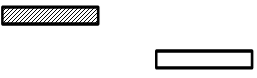
\includegraphics[width=1.5cm,
	keepaspectratio]{img/allen1.png} 	& T1 takes place before T2 \\
	\hline
	T1 &	equals &	T2 &	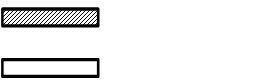
\includegraphics[width=1.5cm,
	keepaspectratio]{img/allen2.png} & T1 is equal to T2 \\
	\hline
	T1 &	meets &	T2 &	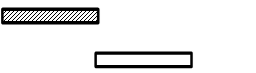
\includegraphics[width=1.5cm,
	keepaspectratio]{img/allen3.png} & T1 meets T2 \\
	\hline
	T1 &	overlaps &	T2 &	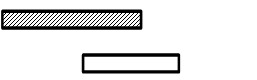
\includegraphics[width=1.5cm,
	keepaspectratio]{img/allen4.png} & T1 starts before T2 and they overlap  \\
	\hline
	T1 &	during &	T2 &	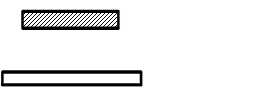
\includegraphics[width=1.5cm,
	keepaspectratio]{img/allen5.png} & T1 is fully contained within T2 \\
	\hline
	T1 &	starts &	T2 &	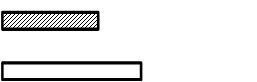
\includegraphics[width=1.5cm,
	keepaspectratio]{img/allen6.png} & T1 starts together with T2 \\
	\hline
	T1 &	finishes &	T2 &	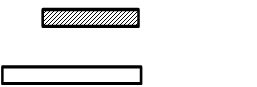
\includegraphics[width=1.5cm,
	keepaspectratio]{img/allen7.png} & T1 finishes together with T2 \\
	\hline
\end{tabular}
\caption[Visual representations of Allen’s temporal relations.]{Visual
representations of Allen’s temporal relations. Adapted
from~\cite{allen_maintaining_1983}.}
\label{table:allen}
\end{table}

Different from previous analyses~\cite{huang_synchronization_1998}, which only
use Allen’s temporal relations for analyzing media objects (output modalities),
we use them for analyzing both output and input modalities. Here, the temporal
interval of an output or input modality means the interval in which it is
activated, \textit{i.e.}~ the time between its activation and its deactivation.

\tab{table:allencomp} presents the analysis of the expressive power of the
selected approaches based on Allen’s temporal relations. In this analysis, for
each relation, we use every possible combination of input modalities (iM) and
output modalities (oM). Some of the works discussed in this \chp{chp:state} were
excluded from the analysis because they do not handle fission and fusion
together. The
excluded works are: the unimodal languages, such as SSML and SRGS; and the
form-based approaches specialized in only one modality, such as VoiceXML, SALT,
and MIML. In addition, we have excluded the HTML-based approaches, because they
lack an explicit specification of synchronization between output and input
modalities, delegating it to JavaScript.

XISL is a form-based language that expresses output modalities (\textit{i.e.}~ system
questions) followed by input modalities (\textit{i.e.}user answers), or
vice-versa. This
means that it is possible to implicitly specify the “iM \textit{meets} oM” and
“oM \textit{meets} iM” relations. Moreover, XISL uses the SMIL operators
(\textit{seq} and
\textit{par}) to combine a set of either output modalities or input modalities
(but not both input and output within a single set). The seq operator in input
modalities enables “iM \textit{meets} iM.” The \textit{seq} operator in output
modalities enables “oM \textit{meets} oM.” The \textit{par} operator in input
modalities enables “iM \textit{starts} iM.” The
\textit{par} operator in output modalities enables “oM” \textit{starts} oM”.
Despite using the SMIL containers, XISL does not offer anchor attributes, such
as \textit{begin} and
\textit{end}, which prevents it from expressing the \textit{before},
\textit{overlaps}, and
\textit{during} relations. Finishes and equals are not supported either.

\begin{table}[!ht]
\scriptsize
%\def\arraystretch{1}
%\resizebox{\textwidth}{!}{%
\begin{tabular}{ m{1.8cm} m{0.5cm} m{1cm} m{0.5cm} m{1cm} m{1cm}
m{1.5cm} m{1.5cm} m{1.5cm}}
	%%%%%%
	\hline
	& \multicolumn{3}{c}{\textbf{Allen’s relation}}
		& \textbf{XISL}	& \textbf{W3C MMI}	& \textbf{SMUIML}	&
		\textbf{SMIL+} \newline \textbf{Rex}	& \textbf{NCL+} \newline
		\textbf{VoiceXML} \\

	%%%%%%
	\hline
	\multirow{7}{*}{fusion}
	& iM &	before &		iM & & & & & \\
	& iM &	equals &		iM & & & Yes & & \\
	& iM &	meets &			iM & Yes & Yes & Yes & &\\
	& iM &	overlaps &	iM & & & & & \\
	& iM &	during &		iM & & & & & \\
	& iM &	starts &		iM & Yes & Yes & Yes & Yes & \\
	& iM &	finishes &	iM & & Yes & & & \\
	\hline

	%%%%%%
	\multirow{7}{*}{fission}
	& oM &	before &		oM & & & & Yes & Yes \\
	& oM &	equals &		oM & & & & Yes & Yes \\
	& oM &	meets &			oM & Yes & Yes & & Yes & Yes \\
	& oM &	overlaps &	oM & & & & Yes & Yes \\
	& oM &	during &		oM & & & & Yes & Yes \\
	& oM &	starts &		oM & Yes & Yes & Yes & Yes & Yes \\
	& oM &	finishes &	oM & & Yes & & Yes & Yes \\
	\hline

	%%%%%%
	\multirow{7}{*}{relating iM-oM}
	& iM &	before &		oM & & & & & \\
	& iM &	equals &		oM & & & & & \\
	& iM &	meets &			oM & Yes & Yes & Yes & Yes & Yes \\
	& iM &	overlaps &	oM & & & & & \\
	& iM &	during &		oM & & & & & \\
	& iM &	starts &		oM & & Yes & & & \\
	& iM &	finishes &	oM & & Yes & & & \\
	\hline

	%%%%%%
	\multirow{7}{*}{relating oM-iM}
	& oM &	before &		iM & & & & & \\
	& oM &	equals &		iM & & & & & \\
	& oM &	meets &			iM & Yes & Yes & & Yes& \\
	& oM &	overlaps &	iM & & & & & \\
	& oM &	during &		iM & & & & & \\
	& oM &	starts &		iM & & Yes & Yes& & \\
	& oM &	finishes &	iM & & Yes & & & \\
	\hline
\end{tabular}
%}
\caption{Multimodal synchronization analysis based on Allen’s relations.}
\label{table:allencomp}
\end{table}

The MMI framework uses the SCXML language to define dialog management, which
provides a state-machine abstraction. SCXML allows synchronizing actions to the
activation and deactivation of states, through the <onentry> and <onexit>
elements. Examples of actions include: the assign action (<assign> element),
which edits the data of an ECMAScript; and the send action (<send> element),
which sends LifeCycle messages to the client application. This way, MMI can
express in a declarative way the starts, finishes, and meets temporal relations.
More specifically: starts may be achieved through Start messages in an <onentry>
element; finishes may be achieved through Cancel messages in <onexit>; and meets
may be achieved through one state sending a Cancel message to an MC in <onexit>,
and another state sending a Start to another MC in <onentry>. MMI cannot express
before, equals, overlaps, and during in a declarative way. Before and equals
would require the use of ECMA script variables and their evaluation in ECMA
script expressions.

The HapticsTK framework uses SMUIML, another state-machine-based language, to
define dialog management. SMUIML, however, does not handle fission and is
limited to sending ad-hoc messages to the client application. Input modalities
may be composed using CARE-based properties: <seq\_and> can express “iM meets
iM”; <par\_end> can express “iM equals iM”; <par\_or> can express “iM starts
iM”. At the end of each relationship, it is possible to send one (“iM meets oM”)
or multiple (“oM starts oM”) ad-hoc messages to the multimedia system.

SMIL and NCL focus on multimedia synchronization and can implement all Allen’s
relations for output modalities. SMIL supports them by using time containers
(seq and par) and their attributes (\textit{e.g.} begin and end). NCL supports them using
causality links and temporal anchors. Therefore, the SMIL+Rex and NCL+VoiceXML
approaches —which extend NCL and SMIL, respectively, with speech modality— also
support Allen’s relation over output modalities.

Regarding input modalities, the SMIL+Rex and NCL+VoiceXML approaches are
limited. SMIL+Rex proposes an <await> element, but it does not support begin and
end attributes. Therefore, the <await> element can be used inside SMIL
containers, but the containers cannot use <await>’s begin and end. The <await>
element and a media inside a seq container enable meets relations between input
and output (“iM followed by iM”, “iM followed by iM”, “iM followed by oM”, “iM
followed by oM”). Additionally, the <await> and a media in a par container
enable starts relations (“oM starts iM” and “oM starts iM”). NCL+VoiceXML maps
the speech recognition inside the VoiceXML onto key-based events in NCL.
This way, it is not possible to activate or de-activate recognizers, and it is
not possible to achieve temporal relation between the activation of input
modalities with other modalities.

\section{Support for multiuser interactions}
\label{sec:state:multiuser}

In this subsection, we discuss works aimed at supporting the development of
multiuser interactions. Illustrated in \tab{table:multiuser}, those works
investigated focus on gaming and DUI (Distributed User
Interface)~\cite{elmqvist_distributed_2011}.

\begin{table}[ht]
\scriptsize
\def\arraystretch{1.5}
\begin{tabular}{ m{3.5cm} m{3cm} m{4.5cm} m{1.3cm} }
	%%%%%%
	\hline
	\textbf{Approach} & \textbf{Application} \newline
	\textbf{specification} & \textbf{User} \newline
	\textbf{abstraction} & Context	\\
	\hline
	%%%%%%
	Microsoft~\cite{microsoft_getting_nodate} and \newline
	Google~\cite{google_supporting_nodate} &
	Imperative \newline (\textit{i.e.}~C\#, Java) &	User
	is a gamepad parameter & Gaming \\
	\hline
	Guerrero-Garcia~\cite{guerrero_garcia_designing_2010} &	UsiXML & User is
	coupled with his/her device & DUI \\
	\hline
	Batista \textit{et al.}~\cite{batista_estendendo_2010,batista_ginga-md:_2013}
	&	NCL & User is coupled with his/her device & DUI \\
	\hline
\end{tabular}
\caption{Comparison among the features supported by the different multiuser
development approaches features.}
\label{table:multiuser}
\end{table}

Microsoft~\cite{microsoft_getting_nodate} and
Google~\cite{google_supporting_nodate} APIs, among other game
APIs, propose multiuser support in gaming contexts. Both enable multiuser
interactions by imperative APIs to handle gamepad controllers. Microsoft
supports multiuser interactions in DirectX applications by the XInput controller
API. Similarly, Google supports multiuser interactions in Android applications
by the gamepad API. Both of these APIs use callback events with an
identification parameter informing the source controller.

UsiXML~\cite{limbourg_usixml:_2005} is a task-oriented GUI description which
adopts an MDE (Model-Driven Engineering) approach to be deployed to different
device configurations (\textit{e.g.} desktop, web, and mobile).
Guerrero-Garcia~\cite{guerrero_garcia_designing_2010} extends UsiXML (USer
Interface eXtended Markup Language) by modeling the coordination of multiple
users in task-oriented systems. In particular, the work models GUIs for group
tasks in UsiXML, in which users or groups of users can interact with one
another. Then, each grouping task is deployed to each device of a user or a
group of users.

Soares \textit{et al.}~\cite{soares_multiple_2009} propose a hierarchical distribution
of media in NCL. The distribution specification uses the abstraction of types of
devices, called device class. The developer of a multimedia application
distributes it by sending and orchestrating the media presentation for the
different device classes. When sending a media (\textit{e.g.} image) to a device class,
Soares \textit{et al.} do not define how the users who interact with the devices can be
identified. Indeed, an expected interaction over a media object in a specific
device class will be triggered when any of the users interact. Soares
\textit{et al.}’s
work —which specified fixed device classes (passive and active)— is extended by
Batista \textit{et al.}~\cite{batista_estendendo_2010,batista_ginga-md:_2013}. In
~\cite{batista_estendendo_2010}, the developers define new device classes using
a description based on the UAProf (User Agent
Profile)~\cite{openmobilealliance_wag_2001} description. In
~\cite{batista_ginga-md:_2013}, they propose that the developer may use a
document variable called child.index, which can be consulted by the developer
inside each NCL document sent to each device.

\section{Drawbacks}
\label{sec:state:drawbacks}

We were able to identify four main drawbacks in the approaches presented in this chapter:

\begin{itemize}
	\item \textit{Lack of support for fine synchronization among modalities.} The
	CARE properties have been used in the fusion process to combine input
	modalities. However, when using audiovisual output modalities in fission
	processes —such as voice synthesizers, videos, or sounds— a multimedia system
	must handle many synchronization issues (\textit{e.g.} lip-sync between a synthesized
	avatar and its speech synthesis). For instance, MMI and HephaticsTK consider
	the multimedia system as a “black box” which, as aforementioned, has the
	drawback of not supporting a fine synchronization between the input and output
	modalities. As stated before, only the approaches based on multimedia
	languages do not suffer this problem.

	\item\textit{Strong encapsulation between fusion and fission.} According to
	Tulk~\cite{turk_multimodal_2014}, one of the main goals of Multimodal
	Interaction research is to enable the development of multimodal systems
	supporting bi-directional communication between humans and machines. However,
	the languages discussed here focus more on supporting either fusion or fission
	processes. On the one hand, the multimedia-based approaches encapsulate the
	fusion process; they delegate the fusion by using scripts (\textit{e.g.} XHTML+VoiceXML)
	or by mapping input modalities to keyboard-based events (\textit{e.g.} NCL+VoiceXML). On
	the other hand, languages such as MMI and SMIUML encapsulate the fission and
	delegate it to a multimedia system (\textit{e.g.} HTML player, in the MMI case).

	\item \textit{Lack of support for modality selection considering sensory
	capabilities.} Modality selection over output modalities is defined as part of
	the fission process \cite{costa_adapting_2011,dumas_multimodal_2009}.
	Such a selection should consider the
	presentation context and the user’s profile (\textit{e.g.} capabilities,
	skills).
	Adapting the input/output media based on human sensory capabilities is an
	issue investigated often by Multimedia research
	~\cite{ghinea_mulsemedia:_2014}. XISL and SCXML propose conditional structures
	—switch and if-then-else, respectively—, which can be used for selecting the
	output modalities. However, they do not support the description of individual
	human sensory capabilities and, as a consequence, they do not directly support
	modality selection based on the users’ sensory capabilities.

	\item \textit{Interacting users are second-class citizens.} For both gaming
	and DUI contexts, the user interaction is identified by the source device, so
	that a user interacting with two devices will be viewed by the system as two
	different users.
\end{itemize}

Schnelle-Walka \textit{et al.}~\cite{schnelle-walka_jvoicexml_2013} discuss the first
two drawbacks when trying to use MMI for implementing a virtual assistant that
helps a user to perform a task. IM implements the virtual assistant using two
MCs: a BML document, for avatar rendering; and a VoiceXML document, for speech synthesis. To
implement their usage scenario, however, they had to violate the MMI
architecture twice. The first violation happened when they had to connect the
BML MC and the VoiceXML MC directly. That was required because the MMI LifeCycle
API does not provide enough support for lip-sync features (in this case, between
the avatar and its speech). Such a workaround shows the lack of support for fine
synchronization in the MMI framework.

According to Schnelle-Walka \textit{et al.}, it is impractical to employ the MMI
framework for synchronizing MCs with continuous output
~\cite{schnelle-walka_jvoicexml_2013}. The second violation occurs when the
virtual assistant IM needs to use an MC for a motion sensor managed by another
IM. MMI defines a tree-based organization of IMs and MCs, which leads to a
strong encapsulation between fusion and fission IM. In other words, the motion
sensor MC, which is used in one of the fusion branches, cannot be (re-)used in
another branch, the virtual assistant one (a fission branch).